\section{Wavefunction and superposition}

A quantum state is described with the help of a wavefunction, which for one dimension we write as

$$\psi(x): \mathbb{R}\rightarrow\mathbb{C} \; .$$

In and of itself the wavefunction does not have a good physical interpretation, but the squared absolute value becomes a probability distribution, such that

\begin{equation}
    P(x) = |\psi(x)|^2 \; ,
\end{equation}

meaning that $|\psi(x)|^2$ is the probability of finding the particle at position $x$. The wavefunction therefor needs to be normalized, such that 

\begin{equation}
    \int_{-\inf}^{\inf}\mathrm{d}x \psi^*\psi = 1 \; .
\end{equation}

It then also means the particle is in a undetermined position before measurement. The quantum state is a combination of all the possible positions it can be in, weighted by $\psi(x)$, in intervals for a continuum of eigenstates $\ket{\phi}$ 

\begin{equation}
    \ket{\psi} = \int\mathrm{d}x \psi(x)\ket{\phi} \; .
\end{equation}

And for a discrete set of eigenstates

\begin{equation}
    \ket{\psi} = \sum_i \psi(x_i)\ket{\phi} \; .
\end{equation}

Such a state $\ket{\psi}$ is called a superposition.

\section{Operators and the Schrödinger equation}

Affecting the wavefunction is done mathematically through operators. An operator maps a state to another, transforming the wavefunction. For a generalized operator $\hat{O}$ and the state $\ket{\psi}$ we have

\begin{equation}
    \hat{O}\ket{\psi} = \ket{\psi'} \; ,
\end{equation}

where $\ket{\psi'}$ is a new state. When an operator acts on a eigenstate:

\begin{equation}
    \hat{O}\ket{\phi} = \varepsilon\ket{\phi} \; ,
\end{equation}

the eigenvalue $\varepsilon$ is a quantity of what $\hat{O}$ represents. For this quantity to be something physically measurable, the operator needs to be hermitian 

\begin{equation}
    \hat{O} = \hc{O} \; ,
\end{equation}

such that $\varepsilon \in \mathbb{R}$. An important observable operator is the hamiltonian, representing the energy of the system. The hamiltonian maps a state to its energy distribution, indicating its time evolution which is dictated by the Schrödinger equation:

\begin{equation}
    i\hbar\frac{\partial}{\partial t} |\Psi(t)\rangle = \hat{H} |\Psi(t)\rangle \; ,
\end{equation}

where $t$ is time. Eigenstates of the hamiltonian are the stable energy states of the system

\begin{equation}
    H\ket{\psi_n} = E_n\ket{\psi_n} \; ,
\end{equation}

where $E_n$ is the energy of the state.

\section{Global and local energy}

The global energy is the energy of the whole system, the possible are values of energy that can be measured. This is the energy eigenvalues of the hamiltonian:

\begin{equation}
    E_n = \frac{\bra{\Psi}H\ket{\Psi}}{\braket{\Psi}{\Psi}} \; .
\end{equation}

For a state:

$$\ket{\Psi} = \alpha_1 \ket{\psi_1} + \alpha_2 \ket{\psi_2} \dots + \alpha_n \ket{\psi_n} \; .$$

For any basis state

$$\ket{\phi} \in \mathbf{B} = \{ \ket{\psi_1, \ket{\psi_2} \dots \ket{\psi_n}} \; ,$$

we have that the local energy is 

\begin{equation}
    E_{\text{local}}(\phi) = \frac{\bra{\phi}H\ket{\Psi}}{\braket{\phi}{\Psi}} \; .
\end{equation}

For a Hamiltonian matrix 

\section{Pauli Exclusion Principle}

The Pauli Exclusion Principle says that, within a quantum system, identical fermions are limited to one per quantum state. This is expressed mathematically with a anti-symmetric wavefunction:

\begin{equation}
    \Psi(\dots,x_i,\dots,x_j,\dots) =-\Psi(\dots,x_j,\dots,x_i,\dots) \; ,
\end{equation}

where $x_i$ and $x_j$ is two particles being switched. To show why this is we look at the simplest cast of only two fermions $x_1$ and $x_2$ with the respective position $\mathbf{r}_1$ and $\mathbf{r}_2$. We have the two states

$$\psi_{12} = \psi_{x_1}(\mathbf{r}_1)\psi_{x_2}(\mathbf{r}_2)$$
$$\psi_{21} = \psi_{x_1}(\mathbf{r}_2)\psi_{x_2}(\mathbf{r}_1)$$

The wavefunction will be a superposition of these two states and we have the symmetric case:

$$\Psi_s = \sqrt{\frac{1}{2}} \left [ \psi_{x_1}(\mathbf{r}_1)\psi_{x_2}(\mathbf{r}_2) + \psi_{x_1}(\mathbf{r}_2)\psi_{x_2}(\mathbf{r}_1) \right ]$$

and the anti-symmetric case:

$$\Psi_a = \sqrt{\frac{1}{2}} \left [ \psi_{x_1}(\mathbf{r}_1)\psi_{x_2}(\mathbf{r}_2) - \psi_{x_1}(\mathbf{r}_2)\psi_{x_2}(\mathbf{r}_1)\right ] \; .$$

To express the Pauli exclusion principle we want to negate the probability of the two fermions being in the same position state, and when we set $\mathbf{r}_1 = \mathbf{r}_2$ we get that:

$$\Psi_s = \sqrt{\frac{1}{2}} \left [ \psi_{x_1}(\mathbf{r}_1)\psi_{x_2}(\mathbf{r}_1) + \psi_{x_1}(\mathbf{r}_1)\psi_{x_2}(\mathbf{r}_1)\right]$$

$$\Psi_a = 0 \; ,$$

we see that the anti-symmetric wavefunction requirement does exactly that.


\section{The bra-ket notation}

For this thesis the bra-ket notation is used to represent states of the vector form. The bra, $\bra{}$, represents a $1 \times N$ matrix:

$$\bra{v} = \begin{bmatrix} v_1 & v_2 & \dots & v_N \end{bmatrix} \; .$$

The ket, $\ket{u}$, represents it as a $N \times 1$ matrix:

$$\ket{u} = \begin{bmatrix} u_1 \\ u_2 \\ \dots \\ u_N \end{bmatrix} \; .$$

With this we have the basic vector-vector multiplication. The inner product is written as:

$$\mathbf{u}^T\mathbf{v} = \braket{u}{v} = \sum_i u_iv_i \; ,$$

and the outer product is written as:

$$\ket{v}\bra{u} = \begin{bmatrix}
  u_{1}v_{1}&u_{1}v_{2}&\dots&u_{1}v_{N}\\
  u_{2}v_{1}&u_{2}v_{2}&\dots&u_{2}v_{N}\\
 \vdots & \vdots & & \vdots \\
 u_{N}v_{1}&u_{N}v_{2}&\dots&u_{N}v_{N} \; .
\end{bmatrix}$$

We want to use this notation to describe a quantum state $\ket{\psi}$. We start with the standard basis, where a system is in a $0$ or $1$ state, often called a qubit:

$$\ket{0} = \begin{bmatrix}
  1 \\ 0
\end{bmatrix} \;\;\;\;\; \ket{1} = \begin{bmatrix}
  0 \\ 1
\end{bmatrix}$$

This means that the system can only be measured to be in state $\left | 0 \right >$ or $\left | 1 \right >$. Before measurement, however, $\ket{\psi}$ can be a superposition of the computational basis states. Which can be described as a linear combination:

$$\left | \psi \right > = \alpha \left | 0 \right > + \beta \left | 1 \right > = \begin{bmatrix}
    \alpha \\ \beta
\end{bmatrix}\; ,$$

where both $\alpha, \beta \in \mathbb{C}$ and with the normalization condition $\lvert\alpha\rvert + \lvert\beta\rvert = 1$. It is usefull to visualize $\ket{\psi}$ as a sphere of possible states it can be in, called the Bloch sphere.

\begin{figure}[H]
    \centering
    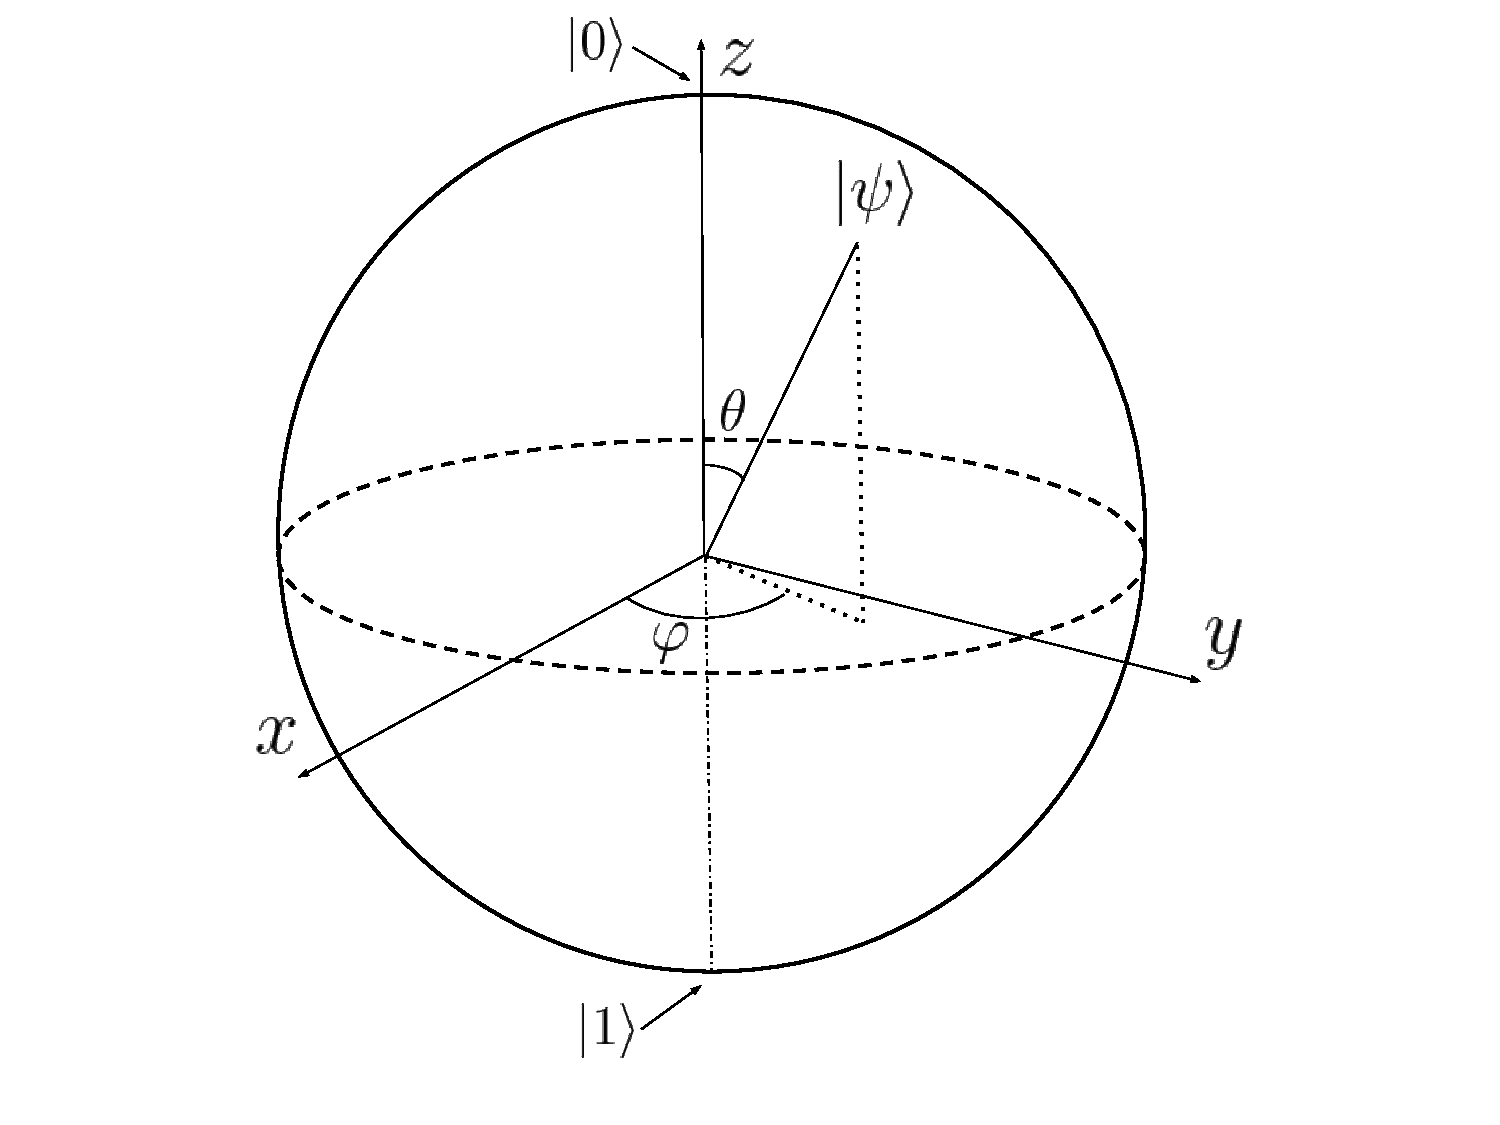
\includegraphics[width=\textwidth]{Figures/Drawn/bloch pshere.pdf}
    \caption{The possible states of a system of a single qubit represented by a sphere with the apexes being the computational basis states.}
    \label{fig:blochsphere}
\end{figure}

Since we have the restriction $\lvert\alpha\rvert + \lvert\beta\rvert = 1$, the two complex values $\alpha$ and $\beta$ only contribute to two degrees of freedom, resulting in the surface of the Bloch sphere, \ref{fig:blochsphere}, as the space of possible states $\ket{psi}$.

\subsection{Multi-Qubit States}

Bringing in another qubit will give us more possible measured outcomes. Therefor our computational basis needs to be expanded, encompassing every possible combination. This is done by tensor product, or Kronecker product, of the possible single qubit measurements. For a two-qubit system we then have

\begin{gather}
\begin{aligned}\label{eq:twoqubit}
    \ket{0} \otimes \ket{0} = \begin{bmatrix} 1 \\ 0 \end{bmatrix} \otimes \begin{bmatrix} 1 \\ 0 \end{bmatrix} &=  \begin{bmatrix} 1 \\ 0 \\ 0 \\ 0\end{bmatrix} \\
    \ket{1} \otimes \ket{0} = \begin{bmatrix} 0 \\ 1 \end{bmatrix} \otimes \begin{bmatrix} 1 \\ 0 \end{bmatrix} &=  \begin{bmatrix} 0 \\ 1 \\ 0 \\ 0\end{bmatrix} \\
    \ket{0} \otimes \ket{1} = \begin{bmatrix} 1 \\ 0 \end{bmatrix} \otimes \begin{bmatrix} 0 \\ 1 \end{bmatrix} &=  \begin{bmatrix} 0 \\ 0 \\ 1 \\ 0\end{bmatrix} \\
    \ket{1} \otimes \ket{1} = \begin{bmatrix} 0 \\ 1 \end{bmatrix} \otimes \begin{bmatrix} 0 \\ 1 \end{bmatrix} &=  \begin{bmatrix} 0 \\ 0 \\ 0 \\ 1\end{bmatrix} \; ,  
\end{aligned}
\end{gather}
which then is a orthonormal basis for our new two-qubit system. To simplify writing, the tensor product between states are often written as

\begin{gather}
\begin{aligned}
    \ket{0} \otimes \ket{0} &= \ket{00} \\
    \ket{1} \otimes \ket{0} &= \ket{10} \\
    \ket{0} \otimes \ket{1} &= \ket{01} \\
    \ket{1} \otimes \ket{1} &= \ket{11} \; .
\end{aligned}
\end{gather}

Adding more qubits is simple. For each additional qubit one uses the tensor product of the current basis with the single-qubit basis, resulting in a doubling of possible states. For a $N$ qubit system we then get $2^N$ possible measured states.
